A possible solution to register a dataset is to select a set of points for each
of the observations and align these points using a warping function. This method
 is called landmark registration.

A landmark, or feature of a curve, is some characteristic that can be
associated with a specific point of the domain. There are typically maximums, minimums or
zero crossings points. For instance, the population shown in Figure
\ref{FIG:LANDMARK} has two distinctive features, formed by the maximum points of
 each of the samples.


\begin{figure}[Shift registration of a dataset]{FIG:LANDMARK}{Shift registration of a dataset}
  \subfigure[SBFIG:LANDMARK1]{Unregistered dataset $f_i(t)$}{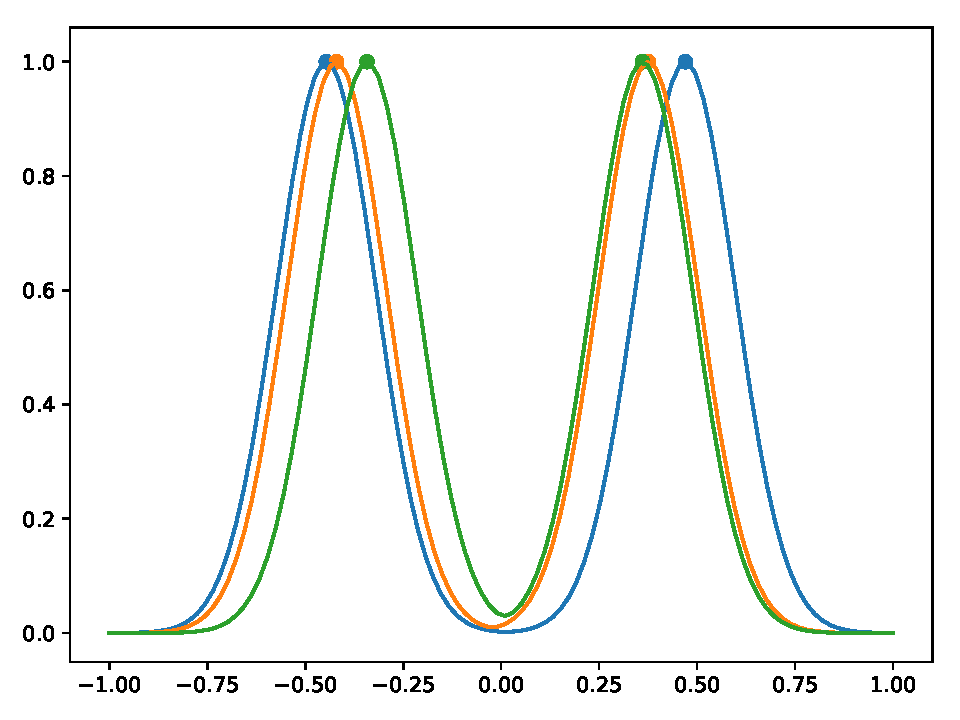
\includegraphics[width=7.5cm]{landmark-dataset}} \quad
  \subfigure[SBFIG:LANDMARK2]{Registered population $f^*_i(t)$}{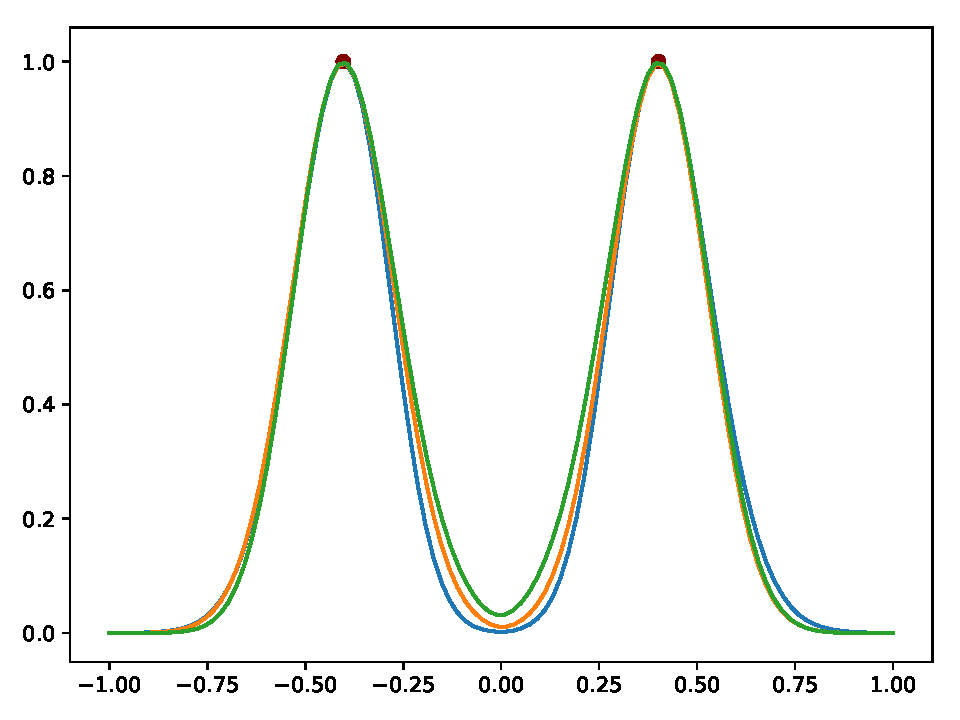
\includegraphics[width=7.5cm]{landmark-registration}}
\end{figure}


The landmark registration process will require, for each observation $f_i$,
the identification of the values $\{t_{ij}\}_{j=1}^{F}$ associated with each of
the $F$ features, which will be aligned to a common point
$\{t_{j}^*\}_{j=1}^{F}$. Once we have the landmarks points, we will build the
 warping functions so that $\gamma_i(t_j^*)=t_{ij}$, thus

\begin{equation}[]{Warping mapping of landmarks}
f_i^*(t_j^*) = f_i(\gamma_i(t_j^*)) = f_i(t_{ij}).
\end{equation}

Not all sets of populations have differentiated characteristics of this type,
moreover, by taking into account only a limited number of points the resulting
alignments can become quite artificial, altering the internal structure of the
samples.
This will motivate us to build methods which use a global criterion for
alignment and not just a discrete number of points.
